
\documentclass[12pt]{article}

\usepackage{graphicx}
\graphicspath{ {./images/} }

\usepackage{epsfig}
\usepackage{amsmath,amsthm}
\usepackage{listings}


\newtheorem{lemma}{Lemma}
\newtheorem{theorem}{Theorem}


\usepackage{titlesec}
\titleformat{\section}
{\normalfont\Large\bfseries}{Question~\thesection:}{1em}{}

\newlength{\toppush}
\setlength{\toppush}{2\headheight}
\addtolength{\toppush}{\headsep}


\def\subjnum{Comp 160}
\def\subjname{Algorithms}


\def\doheading#1#2#3{\vfill\eject\vspace*{-\toppush}%
  \vbox{\hbox to\textwidth{{\bf} \subjnum: \subjname \hfil Erli Cai}%
    \hbox to\textwidth{{\bf} Tufts University, Fall 2020 \hfil#3\strut}%
    \hrule}}


\newcommand{\htitle}[1]{\vspace*{1.25ex plus 1ex minus 0ex}%
\begin{center}
{\large\bf #1}
\end{center}} 



\begin{document}
\doheading{2}{title}{Homework 00}
\setlength\parindent{0pt}

\section{}
(a)\\
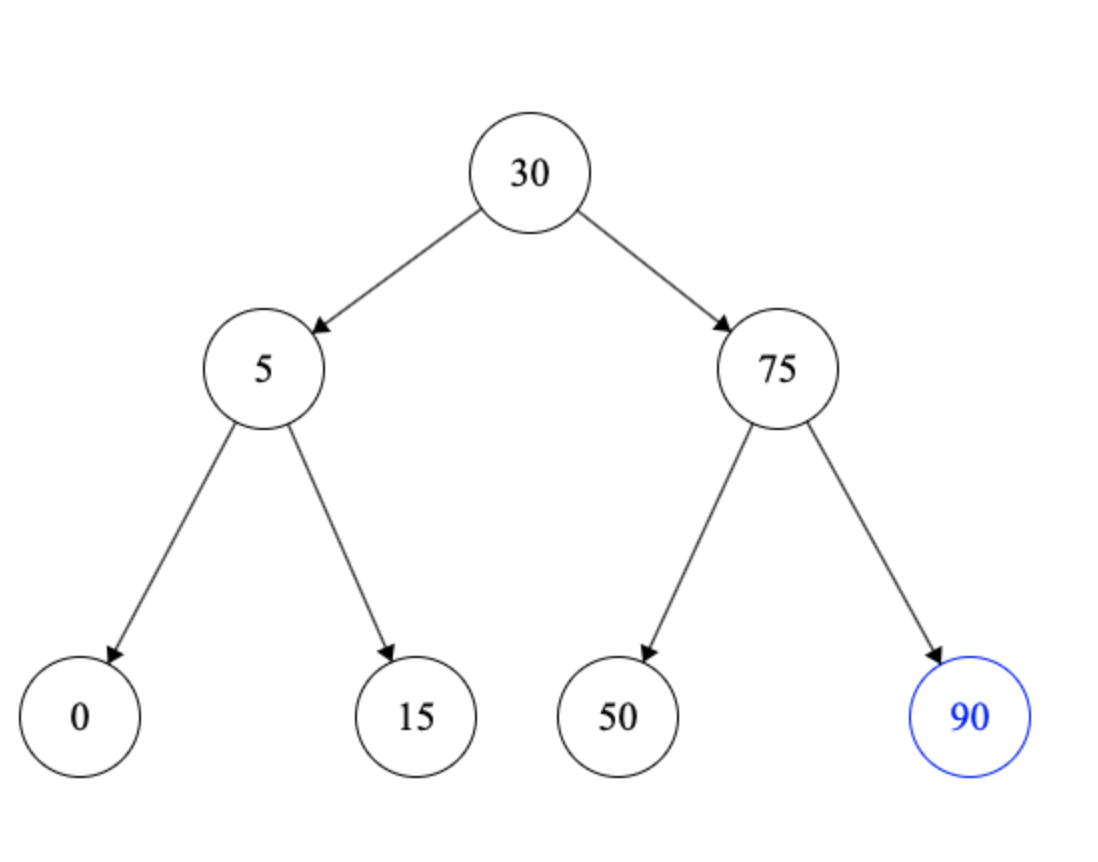
\includegraphics[scale = 0.5]{1}

(b) I will augment the tree with  right endpoint and the largest right endpoint in subtree.\\
Let L, R, maxR be the left endpoint, right endpoint and the largest right endpoint in subtree of the root and . Then steps of the algorithm would be:\\
First check if $L<q<R$, If it is true then q is in the interval of the root and we are done. \\
Otherwise compare L, maxR and q.\\
1) If $q>maxR$, then q is not in any interval.\\
2) If $q<L$, then recurse on the left subtree.\\
3) If $L<q<maxR$ and q is less than the  largest right endpoint in left subtree recurse on the left subtree. Else recurse on the right subtree.\\\pagebreak

(c)\\
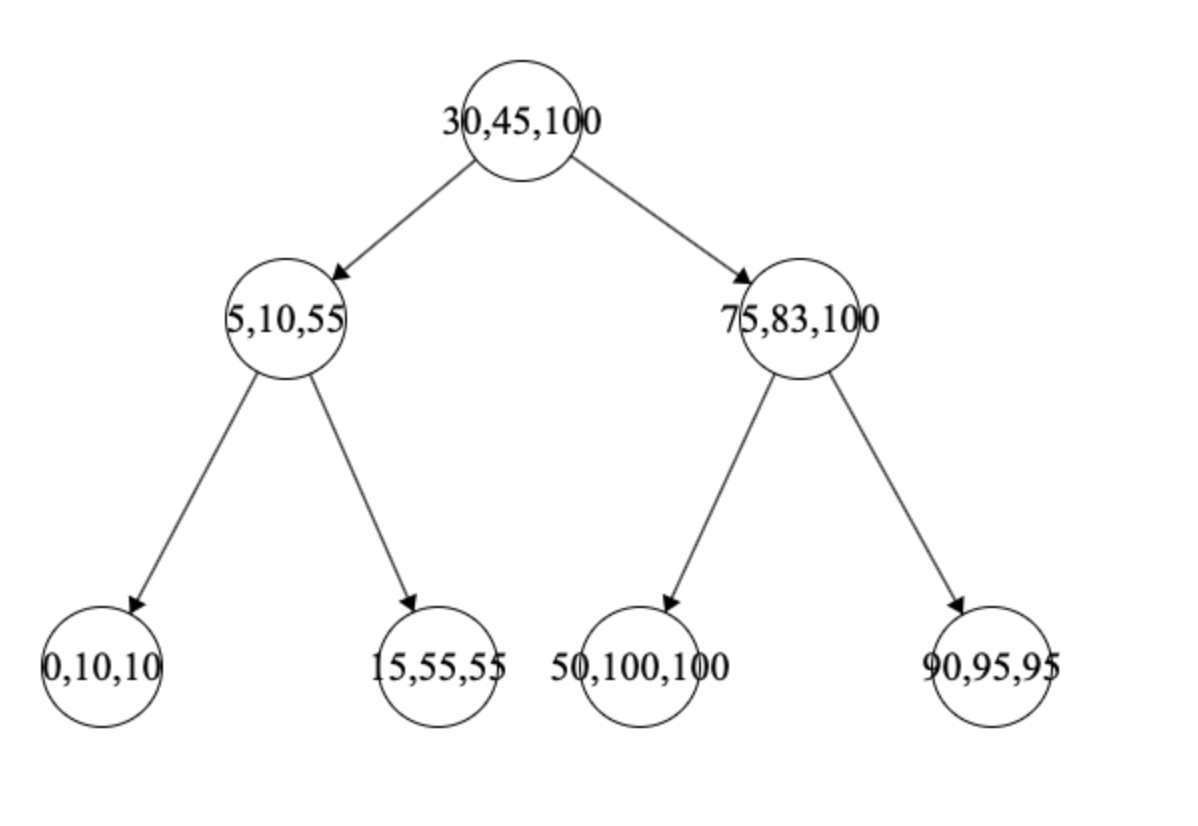
\includegraphics[scale = 0.5]{2}

(d) Yes, We need to modify case (3) in the search algorithm \\
Instead of recursing on either left subtree or the right subtree, we need to check both subtrees in case(3)\\
So case 3) become If $L<q<maxR$ then do apply search algorithm to both left and right subtree.\\
We also need to keep searching the subtree of a node even we have find a answer\\
It will have $\theta(n)$ runtime now.

(e) i.q = 12. $q<30$, so recurse on left subtree.  $5<q<55$, so search in both left subtree and right subtree.\\
In left subtree $10<q$, so no answer. In right subtree$ q<15$, and no left subtree, so no answer\\
In conclusion, 12 is not in any interval.

ii. q = 53. $30<q<100$, so search in both left subtree and right subtree.\\
In left subtree:  $5<q<55$, so search in both left subtree and right subtree. $ 0<q<10$, so no answer in left subtree. $15 <q <55$, so we find an interval.\\
In right subtree: $q<75$, so search in left subtree. $50<q<100$, we find another interval.\\
In conclusion there are two intervals satisfy (15,55), (50,100).\\

My answers make sense
\pagebreak
\section{}
In the following answer, I writer MULTIPOP(k) as Multipop k elements.
(a)worst-case runtime of a single Multipop operation is $\theta(n)$ where n is the length of the stack\\

(b) At most n elements are pushed into the array in n operations. And each elements get in and gets out of the array in 2 steps. So roughly speaking it takes 2n (or we can say$\theta(n)$) time\\

(c) 2 virtual cost for each PUSH operation and 0 virtual cost for POP and MULTIPOP\\
Real cost: PUSH and POP takes 1 step and MULTIPOP(k) takes k steps.\\

(d) When an element is pushed into the stack, it deposit 2 coins and only use 1. So it has net gain 1 coin.\\
Multipop(k) takes k operations, so on average poping takes 1 coin for each element using multipop, which is the net gain when that element is pushed into the array. Therefore the number of coins remaining would never go negative. And POP can be think of as MULTIPOP(1), so it is also true for POP.\\

(e) PUSH deposit most coins among different operations .And in n operations, we have at most n PUSH operations, so we deposit at most 2n coins. Therefore, n operations takes $\theta(n)$ time.\\

(f) Yes. MULTIPUSH k elements can think of pushing k elements one at each time, so it will have k times the deposit coins of PUSH. So n operations will now take $\theta(kn)$ ime

\pagebreak
\section{}
(a) I want to implement this with an array\\

(b) Insert(S,x) will insert at the end of the array. each operation would take O(1) step.\\

(c) Suppose we now have n elements in the array S. we first use merge sort on S, this takes O(logn) time. And then delete the larger half of the array, which takes O(1) time.\\
So Delete-Half(S) would take O(log n)time.\\

(d) number of elements in the array.\\

(e) $\Phi = 2 \#$(elements in S). Potential of an empty data structure is 0\\

(f) For an insertion, $\hat{c}_i = 1 + \Phi_{i} - \Phi{i-1} = 1+ 2 =3$\\
For Delete-Half,   $\hat{c}_i = \log{n}  + \Phi_{i} - \Phi{i-1} = \log{n}-n \le 0$\\
So,  the amortized cost of any operation cˆ is constant.\\

(g) If $\hat{c}_i  = O(1)$, then m operations would have amortized runtime\\
$\Sigma_{i=1}^{i=m}\hat{c}_i = m \times O(1) = O(m)$ time






\end{document}


